

\documentclass[crop,tikz]{standalone}
\usetikzlibrary{fit, positioning, calc, shapes, shapes.geometric, arrows, arrows.meta}
\tikzset{
  big edge/.style={green, thick,},
  big edgec/.style={big edge, -{Bar[fill=green,green,width=4,length=0,sep=0]}},
  big region/.style={draw, rectangle, rounded corners=1.5, dashed, dash pattern=on 1pt off 1pt, thin, gray,},
  big site/.style={big region, fill=gray!60, text=black,},
  big react/.style={black, thick, -stealth, line width=3, shorten <=3, shorten >=3,},
  big react rev/.style={black, thick, stealth-stealth, line width=3, shorten <=3, shorten >=3,},
  big inst map/.style={thick, -stealth, blue, dashed},
  lbl/.style={font=\tiny\sf, inner sep=1,},
  lbl conc/.style={font=\tiny, inner sep=1,}
}
\usepackage{amsmath,amssymb}
\DeclareMathOperator{\react}{\mathrel{\frac{\raisebox{0.75mm}{\begin{scriptsize}\ensuremath{\hspace*{1mm}\ \hspace*{1mm}}\end{scriptsize}}}{}} \joinrel{\!\!\vartriangleright}}
\newcommand{\reactp}[1]{\operatorname{\mathrel{\frac{\raisebox{0.75mm}{\begin{scriptsize}\ensuremath{\hspace*{1mm}\ #1 \hspace*{1mm}}\end{scriptsize}}}{}} \joinrel{\!\!\vartriangleright}}}
\DeclareMathOperator{\rrul}{\mathrel{\frac{\raisebox{0.75mm}{\begin{scriptsize}\ensuremath{\hspace*{1mm}\ \hspace*{1mm}}\end{scriptsize}}}{}} \joinrel{\!\!\blacktriangleright}}
\newcommand{\rrulp}[1]{\operatorname{\mathrel{\frac{\raisebox{0.75mm}{\begin{scriptsize}\ensuremath{\hspace*{1mm}\ #1 \hspace*{1mm}}\end{scriptsize}}}{}} \joinrel{\!\!\blacktriangleright}}}
\newcommand{\rrula}[2]{\operatorname{\mathrel{\frac{\raisebox{0.75mm}{\begin{scriptsize}\ensuremath{\hspace*{1mm}\ #1 \hspace*{1mm}}\end{scriptsize}}}{\begin{scriptsize}\ensuremath{\hspace*{1mm}\ #2 \hspace*{1mm}}\end{scriptsize}}}\joinrel{\!\!\blacktriangleright}}}

\begin{document}

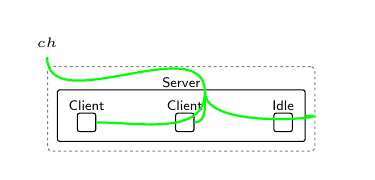
\begin{tikzpicture}[
  ,
_BIG_server/.append style = {draw, rounded corners=0.8},
_BIG_idle/.append style = {draw, rounded corners=0.8},
_BIG_client/.append style = {draw, rounded corners=0.8}
  ]
    
\node[_BIG_client,  label={[inner sep=0.5, name=n1l]north:{\sf\tiny Client}}] (n1) {};
\node[_BIG_client, right=1.00 of n1, label={[inner sep=0.5, name=n2l]north:{\sf\tiny Client}}] (n2) {};
\node[_BIG_idle, right=1.00 of n2, label={[inner sep=0.5, name=n3l]north:{\sf\tiny Idle}}] (n3) {};
\node[_BIG_server, fit=(n3)(n3l)(n2)(n2l)(n1)(n1l), label={[inner sep=0.5, name=n0l]north:{\sf\tiny Server}}] (n0) {};
\node[big region, fit=(n0)(n0l)] (r0) {};
\node[] at ($(r0.north west) + (0,0.3)$) (name_ch) {\tiny $ch$};
\coordinate (h0) at ($(n0) + (0.3,0.3)$);
\draw[big edge] (n0) to[out=0,in=-90] (h0);
\draw[big edge] (n1) to[out=0,in=-90] (h0);
\draw[big edge] (n2) to[out=0,in=-90] (h0);
\draw[big edge] (name_ch) to[out=-90,in=90] (h0);

\end{tikzpicture}
  
\end{document}
